\documentclass[12pt]{article}

\usepackage{hyperref}
\usepackage{titlesec}
\usepackage{amsthm,amssymb}
\usepackage{amsmath}
\usepackage{graphicx}
\usepackage{minted}

\graphicspath{ {images/} }

\title{CS3210 Assignment 1 Report}
\date{\today}
\author{Mok Wei Xiong, Edmund (A0093960X)}

\begin{document}
% title
\maketitle

\section{Program Design}

\subsection{General Description}
In my design, a train is represented by a thread. If there are $n$ trains in total for all green, yellow and blue lines, then there will be $n$ threads representing the trains. Additionally, in the simulation, I will also have $1$ thread (the master thread) that does not represent any train, but is in charge of printing the state of the trains at every tick. Thus, during the simulation, if there are a total of $n$ trains in the system, there will be $n+1$ threads.

\bigbreak \noindent Every thread is in charge of only $1$ train, and controls that train throughout the entire simulation. Each thread will loop for $N$ iterations, where each iteration represents a tick. In each iteration, each thread will attempt to load people into the train, move along a track, or just do nothing if it is waiting for another train in front of it. Named critical sections are used as mutexes to prevent race conditions by trains waiting for the same station, or trains waiting for the same track. FIFO Queues are similarly used at each station and track to prevent starvation, by guaranteeing that any train that is queued will be eventually served.

\subsection{Assumptions}
\begin{itemize}
	\item We are given that only one train can load at a station (for a given direction) at any time. There can be multiple trains waiting at a station. Once the first train is done loading, it may possibly still have to wait for another train on the track in front of the station before it is allowed to leave. I assume that the train behind can be allowed to start loading, meaning it can open the door to load passengers, even though the first train may still be waiting for the track.
	\item The definition of \textbf{average waiting time} given in the assignment handout is not very clear on whether the average waiting time is (A) the average of all individual average waiting times of each station on a line, or (B) the average of \textit{all} waiting times experienced by every station on the line. I have chosen to take approach (B) for my implementation.
\end{itemize}

\section{Implementation Details}

\subsection{Stations on a line}

The input format given specifies three lines $G, Y, B$, with each line containing a list of stations separated by commas to indicate the stations that are served by each of the lines. The sample format nicely specifies each list of station in "order", where the terminal stations are at the start and end of the list, and the stations in between connect the two terminals. For example, the input format specifies, for the yellow line, \verb!tuas, clementi, tampines, changi!, which is a right "order" for the line, whereas an input format that does not specify a right order is something like \verb!clementi, tampines, tuas, changi!.

\bigbreak \noindent In my implementation, I do not assume that the input format will always supply the list of stations in "order", but instead attempt to put the stations in order in a straight line. This way, even if the input format gives the stations in a random order, I will always be able to find an "order" and my trains will be added to the right terminal stations.

\bigbreak \noindent This is done using a simple search for a terminal station (only one outgoing "edge" for the specified line), and then traversing its unvisited neighbour until the other terminal station is reached.

\subsection{Integer loading times}

The input popularities for each station is specified as a floating point number, which means that the loading times should also be a floating point number. However, the simulation works in discrete time ticks, so it would not be possible to perform actions like stopping the train from loading between two integer time ticks, once the loading time is up. Thus, I took the ceiling for each loading time computed using \verb!ceil! so that the train will always wait at least the correct amount of time to load.

\subsection{Train threads}

As mentioned, for every train in the simulation, there will be a thread that is spawned and in charge of that train throughout the entire simulation. Before the simulation, a vector of \verb!Train! objects are created, and the master thread will feed appropriate information into each \verb!Train! so that later during the simulation, each thread will know the current state of its \verb!Train! using only its allocated \verb!Train!. Examples of what each \verb!Train! contains include what line it is in, the train number, the stations in this line, the direction it is moving in, and whether it is currently loading or moving. The \verb!thread_id! of each thread is used to identify the \verb!Train! that the thread is assigned to.

\bigbreak \noindent The threads are created using \verb!#pragma omp parallel num_threads(n + 1)!, where n is the total number of trains in the system. There is an additional $1$ thread that will not be in charge of any train and simply prints the state of every train at each tick.

\subsection{Synchronization}

\subsubsection{Printing state}

\begin{minted}{C++}
  #pragma omp parallel num_threads(train_counts.num_total + 1)
  {
    // master will occupy thread_id = 0, so offset all workers by 1
    int thread_id = omp_get_thread_num();
    int train_id = thread_id-1;

    // Run for max_tick number of times
    for (int tick=0; tick<max_tick; tick++) {

      // First let master print out the current state of the system
      #pragma omp master
      {
        print_system_state(trains, tick);
      }

      // Let master finish printing before all trains make their moves
      #pragma omp barrier

      // All trains make their move for this tick
      // (except master thread who does not own a train)
      if (thread_id != MASTER_THREAD) {
        Train& train = trains[train_id];
        assert(train.gnum == train_id);
        simulate_train(train, tick);
      }

      // Let all trains wait for master to print their state
      #pragma omp barrier
    }
  }
\end{minted}

\bigbreak \noindent The above code snippet shows the synchronization structures used to ensure that there is no race condition when the master thread attempts to print the state of the system in the current tick.

\bigbreak \noindent In each tick, the master thread will always get to print the system state before every other train makes its move for the current tick. This is ensured by the usage of the \verb!#pragma omp barrier! after the code used to get the master to print the system state within \verb!#pragma omp master!. Only when the master has completed printing the state, will all the threads pass through the first barrier. After that, every train will make its move for the current tick using \verb!simulate_train!. Another \verb!#pragma omp barrier! is placed at the end of the current tick to make sure all trains have finished making their move for the current tick before proceeding on to the next tick, to prevent race conditions.

\subsubsection{Queueing trains}

At every station and every track connecting two stations (in a single direction), there will be a queue. Trains must queue up to load passengers, or start moving on a track using the respective queues before they are allowed to take action. They can only take action when they are at the front of the queue.

\bigbreak \noindent This queue prevents starvation since the moment any train arrives at a station or a track, it is immediately enqueued into the appropriate queue and waits for its turn in the queue. Since the train at the front of the queue will eventually complete, since there is a limit to the time the train at the front of the queue can load passengers or move across a track, it will eventually be removed from the front of the queue. This means every train in the queue will eventually reach the front of the queue where it is then allowed to execute its appropriate action, and thus there will not be starvation!

\subsubsection{Synchronizing queues}

Since we are using the front of the queue to determine whether the train is allowed to take action, there is a possibility of a race condition, affecting the outcome depending on whether the train at the front of the queue executes before the train just behind the front of the queue, or after. In order to avoid this race condition, I use a \verb!#pragma omp critical(name)!, to act as a mutex so that only one thread interested in \verb!name! can manipulate the queue at any time. In the case of station mutexes, \verb!name! is a concatenation of \verb!direction! (either \verb!FORWARD! or \verb!BACKWARD!) and the station number. In the case of track mutexes, \verb!name! is a concatenation of the \verb!source! station and the \verb!destination! station.

\subsection{Simulation Ticks vs Execution Time}

This implementation of the simulation used discrete time units (ticks) instead of running based on execution time.

\bigbreak \noindent There are several advantages of this approach:
\begin{itemize}
	\item Waiting times do not depend on CPU power when using ticks. For every tick, waiting times do not depend on how fast the CPU takes to execute that tick. This means that we can compare waiting times across different CPUs, and even different number of threads on the same CPU (especially very large number of threads for very large number of trains), because the context switching will not impact the waiting times.
	\item Ease of implementation. Implementation is easier when every thread only needs to deal with a single tick, and determine what it should do during that tick. If ticks were not used, we may need things like sleep timers (for example, to sleep until the load time at a station has expired, or to sleep until the train has completed using a track), or more synchronization primitives like condition variables (to know when the train ahead has finished loading, or finished using a track, and the next train can start doing something). With ticks, we can just check if these conditions are met in the current tick.
	\item Simulation time units are also not affected by \verb!IO!, which occurs quite frequently in this simulation (every tick the master thread does some \verb!IO! to print the state of the syem).
\end{itemize}

\bigbreak \noindent However, there are also downsides:
\begin{itemize}
	\item Since the popularities of each station can be a floating point number, according to the loading time formula, the loading time for a train can also be a floating point number. However, since the simulation uses single integer ticks, the simulation will force the train to continue loading until the next nearest integer (ceiling), which means that the simulation will lose its accuracy here when computing the average, minimum and maximum waiting times.
\end{itemize}


\section{Execution Times}

Each execution time result is obtained by running the programme $5$ times, and taking the minimum execution time across all runs. All runs were executed on Dell Precision 7820 with Intel Xeon. Each run used the same system as provided in the assignment handout, but with $N$, the number of time-ticks for the simulation set to $1000$. The program was compiled using \verb!g++ -std=c++11 main.cpp -fopenmp -O3 -o main!, and each test case was placed in a file \verb!example.in! in the same directory. Each run was executed by using \verb!time ./main < example.in!, and the resulting \verb!real! time output was considered as the execution time.

\begin{table}[]
\begin{tabular}{|l|l|l|}
\hline
Number of trains & Composition (G,Y, B) & Execution Time (seconds) \\ \hline
1                & 1, 0, 0              & 0.015                    \\ \hline
2                & 1, 1, 0              & 0.016                    \\ \hline
3                & 1, 1, 1              & 0.017                    \\ \hline
6                & 2, 2, 2              & 0.023                    \\ \hline
10               & 3, 3, 4              & 0.042                    \\ \hline
15               & 5, 5, 5              & 0.053                    \\ \hline
18               & 6, 6, 6              & 0.054                    \\ \hline
19               & 7, 6, 6              & 0.082                    \\ \hline
20               & 7, 7, 6              & 0.173                    \\ \hline
25               & 8, 8, 9              & 0.22                     \\ \hline
30               & 10, 10, 10           & 0.259                    \\ \hline
35               & 12, 12, 11           & 0.313                    \\ \hline
40               & 14, 14, 12           & 0.335                    \\ \hline
50               & 16, 16, 18           & 0.45                     \\ \hline
64               & 20, 20, 24           & 0.593                    \\ \hline
\end{tabular}
\caption{Result of execution time across number of trains}
\end{table}

\begin{figure}
	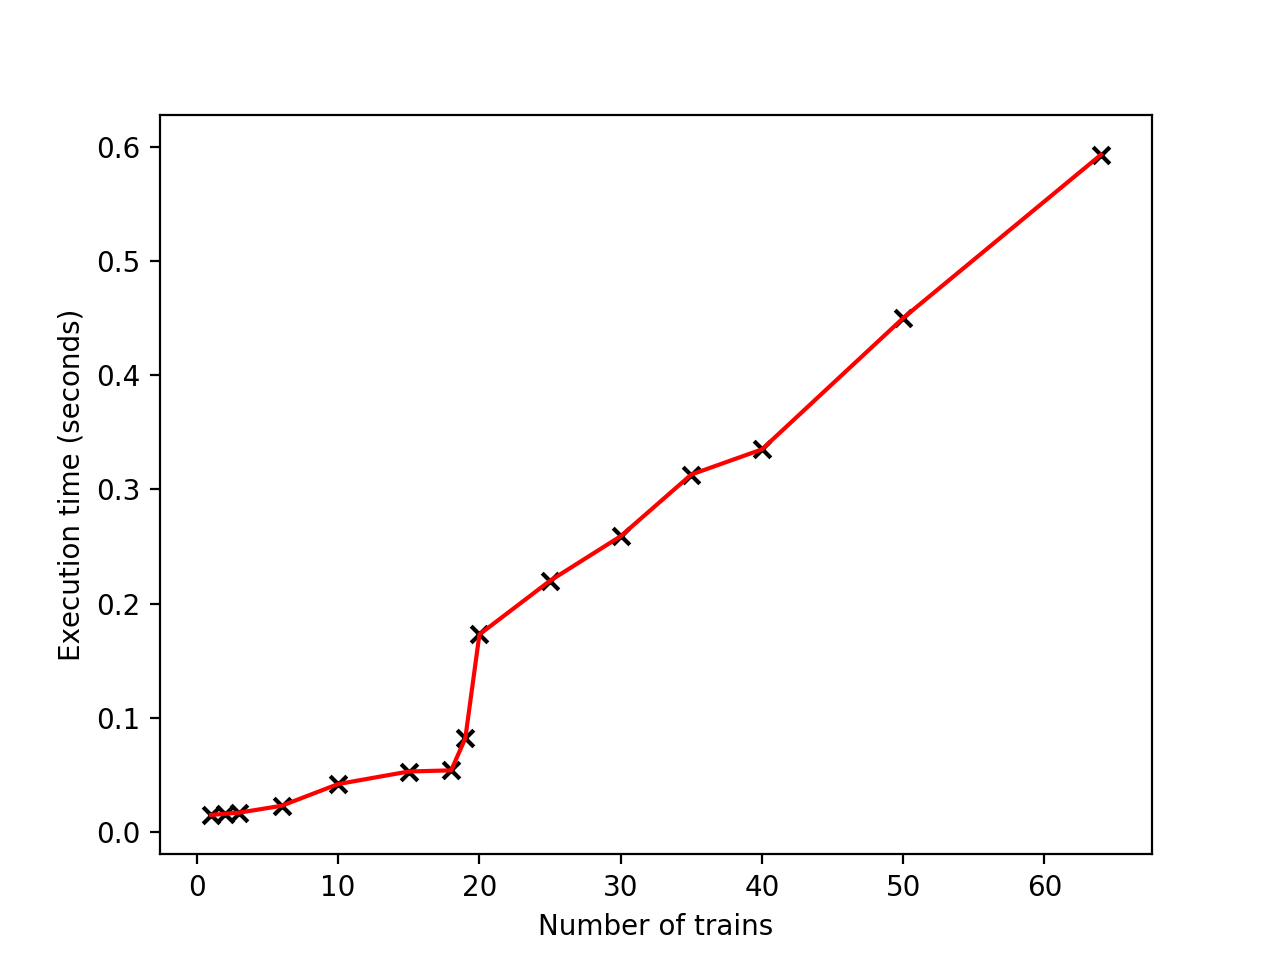
\includegraphics{execution_times}
	\caption{Plot of execution time across number of trains}
\end{figure}

\section{Result Analysis}

\subsection{General trend}

In general, from the plot and the table, we can observe that the execution times increase with increasing number of trains (threads). 

\bigbreak \noindent There are a couple of possible reasons for this:
\begin{itemize}
	\item More trains means more context switching between different threads, which leads to overhead resulting in higher execution time.
	\item More trains means that the master thread needs to loop through more trains in each tick to print out more train states during each tick. This means that there is more \verb!IO! with increasing number of threads, which can be quite slow and thus lead to greater execution times.
	\item More trains means more competition for critical sections. If a thread fails to enter a critical section, it has to wait until it gains access before it can proceed with the rest of the code. Since more competition for critical sections results in a higher chance of failure in gaining access to critical sections, more threads are delayed in completing their work for the current tick, thus increasing execution times per tick, and hence over the entire simulation.
\end{itemize}

\subsection{Mysterious Spike}

Besides the general increasing trend, we can notice an obvious mysterious spike in execution time at around $20$ trains, or $20$ threads. I suspected that it had something to do with the number of cores on the Intel Xeon processor, and the maximum number of threads the Xeon processor could handle optimally. Even if the Intel Xeon had multiple cores, the general advice is to have a maximum of $2$ threads per core for optimal performance before the increasing number of threads begins to hurt performance.

\bigbreak \noindent I referred to Part 2 of Tutorial 1's handout, where we were given a diagram of the workbench cluster. In the diagram, specifications of the Intel Xeon used were given - 10 cores (20 threads)! Just as I had suspected, beyond 20 threads, the Xeon processor cannot perform as well as the number of threads per core started becoming suboptimal. 

\bigbreak \noindent The last observation is that the rate of increase after the spike is greater than before the spike. I think the possible reasons for this are similar to before: the overhead in context switching between threads, the greater competition for critical sections between threads.

\section{Bonus}

As mentioned in section 2.4.2, I believe that my implementation will never encounter starvation since every train that wants to wait for a resource will be doing so in a queue, and train will always reach the front of the queue eventually. As a result, the train will eventually get to execute its action and will never starve. The train at the front of the queue will always leave the queue eventually because the time it can be at the front of the queue is finite and bounded, so trains at the back of the queue can eventually move to the front.

\end{document}
